\documentclass[11pt,a4paper]{article}

\usepackage[margin=1in]{geometry}
\usepackage{amsmath,amssymb,amsfonts}
\usepackage{graphicx}
\usepackage{booktabs}
\usepackage{hyperref}
\usepackage{xcolor}
\usepackage{bm}
\usepackage[numbers,sort&compress]{natbib}


\newcommand{\diag}{\mathrm{diag}}
\newcommand{\eff}{\mathrm{eff}}
\newcommand{\anc}{\mathrm{anc}}
\newcommand{\rec}{\mathrm{rec}}
\newcommand{\true}{\mathrm{true}}
\newcommand{\FR}{\mathrm{FR}}
\newcommand{\sQ}{s^{Q}}
\newcommand{\sC}{s^{C}}

\providecommand{\ket}[1]{\left|#1\right\rangle}
\providecommand{\bra}[1]{\left\langle#1\right|}

\title{The OneBitHHL quantum filter for segment-level track finding in a planar LHCb~VELO toy:\\
algorithm, padding, spectral kernel, and the $\gamma=3$ rejection notch}

\author{Internal report --- Quantum Track Reconstruction working note\\
\small Nikhef / Vrije Universiteit, Amsterdam}
\date{\today}

\begin{document}
\maketitle

\begin{abstract}
We document the one-bit phase-estimation linear-solver variant (\textsc{OneBitHHL} /
\textsc{OneBQF}) used for segment-level track finding in the planar LHCb~VELO toy
\texttt{lhcb\_velo\_toy} (v2.0.0). The Hopfield-style segment Hamiltonian, the cost
function, the choice of $\varepsilon$, $\gamma$, $\delta$, and the segment activation
threshold $\tau$ are stated explicitly. The action of \textsc{OneBitHHL} is derived as a
\emph{spectral filter} $f(\lambda) = \cos(\pi\lambda/(2c))$ with $c = \gamma + \delta$;
this is shown to differ qualitatively from the matrix inverse delivered by HHL. With the
nominal classical operating point ($\gamma=3$, $\delta=1$, $\varepsilon = 2\,\mathrm{mrad}$,
$\tau = 0.35$, $\sigma_{\mathrm{res}} = 5\,\mathrm{\mu m}$, $\sigma_{\mathrm{scatt}} =
0.1\,\mathrm{mrad}$, $1\%$ random hit drop), the spectrum of $A$ straddles the rejection
notch at QPE phase $\varphi = 0.5$ and one quarter of the eigenmodes are completely
wiped. At low track multiplicities ($T \le 10$) this manifests as a $\eff_Q
\approx 0.73$ efficiency floor; at high multiplicities ($T \ge 200$) the same kernel
inflates the false-segment activation count by up to a factor four, producing a
runaway false rate even at exact-statevector readout. A post-processing threshold sweep
shows that raising $\tau$ from $0.35$ to $0.40$ suppresses the high-$T$ false rate from
$\approx 55\%$ to $\approx 1\%$ at $T = 500$ and from $\approx 83\%$ to $\approx 0\%$ at
$T = 1000$, at a $0.5\text{--}4\%$ efficiency cost. Statevector ($E_1$) and finite-shot
sampling ($E_2$) readouts agree within $1\%$ at every $T$ in the sweep, ruling out
shot noise as the failure mode.
\end{abstract}

\section{Introduction}
\label{sec:intro}
The \texttt{lhcb\_velo\_toy} package generates planar VELO events and reconstructs tracks
via two equivalent routes: an inner triplet-cone segment graph passed to either a sparse
linear solver (the ``classical'' route) or to a quantum linear-system algorithm. This
note characterises the second route and stands alongside the classical-only segment-level
report~\cite{velo_toy}. A companion document compares the two solvers head-to-head; here
we restrict ourselves to defining the algorithm, identifying its failure modes, and
demonstrating that they are not statistical artefacts.

\section{Event model and reconstructable-track definitions}
\label{sec:event}
\begin{description}
\item[Geometry.] Five planar modules at $z \in \{33, 66, 99, 132, 165\}\,\mathrm{mm}$;
half-width $40\,\mathrm{mm}$; PV uncertainty $\sigma_{PV} = (0,0,1)\,\mathrm{mm}$; opening
cone $\phi_{\max} = \theta_{\max} = 0.2\,\mathrm{rad}$; particle: pion.
\item[Detector effects.] Hit-position resolution $\sigma_{\mathrm{res}} = 5\,\mathrm{\mu m}$;
multiple-scattering angle $\sigma_{\mathrm{scatt}} = 10^{-4}\,\mathrm{rad}$; random hit drop
$p_{\mathrm{drop}} = 0.01$.
\item[Reconstructable track.] At least three reconstructable hits remaining after the
drop; matched-hit purity $\ge 0.70$; minimum hit efficiency $0$ (LHCb default).
\end{description}

\section{Segment graph and the Hopfield Hamiltonian}
\label{sec:ham}
Triplets of hits $(h_a, h_b, h_c)$ with $h_a, h_b, h_c$ on consecutive modules are
collected; the central hit $h_b$ defines a \emph{segment node} whose direction is the unit
vector along $\vec{h_b - h_a}$ stitched with $\vec{h_c - h_b}$. Two segment nodes $i, j$
sharing the central hit $h_b$ are connected by an edge if the angle between their
direction vectors is below the tolerance $\varepsilon$, equivalently $\cos\theta_{ij} >
\cos\varepsilon$. The total number of segment nodes scales empirically as $N_s \sim T^p$
with the fitted exponent $p$ stable at $3.93$ for $T \in [2,5]$ falling to $3.91$ at
$T = 1000$~\cite{velo_toy}.

The activation amplitude $s \in \mathbb R^{N_s}$ minimises
\begin{equation}
\label{eq:cost}
\mathcal H(s) \;=\; \tfrac{1}{2} s^{\top} A\, s \;-\; b^{\top} s, \qquad
A = (\gamma + \delta)\, \mathbb 1 - W, \qquad
b = \delta \cdot \mathbb 1_{N_s},
\end{equation}
with $W \in \{0,1\}^{N_s \times N_s}$, $W_{ij} = 1$ if and only if segments $i,j$ share a
hit and pass the $\varepsilon$ alignment cut~\cite{stimpfl_garrido}. Symmetry is enforced by
$W \leftarrow W + W^{\top}$ and the diagonal set to $0$. Because $A$ is real symmetric
with strictly positive diagonal $(\gamma+\delta)$ and unit off-diagonals limited to the
shared-hit neighbourhood, $A$ is SPD for the parameter choices considered here. The
classical solver returns $s^* = A^{-1} b$; the quantum solver of
Section~\ref{sec:onebithhl} returns a spectrally filtered approximation.

\paragraph{Parameter choices.}
The base values used throughout this report are
\begin{equation}
\gamma = 3, \quad \delta = 1, \quad \varepsilon = 2\,\mathrm{mrad} \text{ (fixed override)}, \quad
\tau = 0.35.
\end{equation}
The values of $\gamma, \delta, \tau$ are the §14e operating point of
\texttt{segment\_level\_analysis.ipynb}~\cite{Funke2025}. The $\varepsilon$ override
(replacing the formula-driven $\varepsilon \sim 2\sigma_{\mathrm{scatt}}$) is deliberate
and applied identically on the classical and quantum sides for direct comparability.

The two Hopfield fixed-points relevant for the activation threshold are the false-segment
attractor $\delta/(\gamma+\delta) = 0.25$ and the outer-truth attractor at $0.36$; the
choice $\tau = 0.35$ sits between them.

\section{The OneBitHHL spectral filter}
\label{sec:onebithhl}

\subsection{Padding and Hamiltonian simulation}
The pair $(A,b)$ is padded to dimension $N = 2^n$, $n = \lceil \log_2 N_s \rceil$; the
right-hand side is padded with ones, then normalised, $\ket{b} = b_\mathrm{pad}/\|b_\mathrm{pad}\|_2$.
Provided the diagonal is strictly constant $c = \gamma + \delta$ (true by construction
for the unmodified \textsc{SimpleHamiltonianFast}), the time-evolution factorises
$e^{-iAt} = e^{-ict} e^{+iBt}$ with $B = c\mathbb 1 - A$ off-diagonal. Each unit
off-diagonal entry is implemented as a multi-controlled $\mathrm{RX}(2t)$ Givens
rotation; with the choice
\begin{equation}
\label{eq:t}
t \;=\; \pi / c \;=\; \pi/(\gamma+\delta),
\end{equation}
the evolution is exact (no Trotter step).

\subsection{Phase estimation, X--CX--X gadget, and the cosine kernel}
With one time qubit, QPE produces the entangled state
\begin{equation}
\ket{\Psi} \;=\; \sum_k \beta_k \big[\,\cos(\pi\varphi_k)\,\ket{0}_t
                 \;-\; i\sin(\pi\varphi_k)\,\ket{1}_t\big]\ket{\lambda_k},
\quad \varphi_k = \lambda_k / (2c),
\end{equation}
where $\ket b = \sum_k \beta_k \ket{\lambda_k}$ expands in the eigenbasis of $A$.
The standard HHL ancilla rotation is replaced by $X_t\,\mathrm{CX}_{t\to a}\,X_t$:
post-selecting the ancilla on $\ket 1$ keeps exactly the time-qubit-$\ket 0$ branch.
Uncomputing QPE returns the system register, modulo the post-selection probability, to
\begin{equation}
\label{eq:kernel}
\ket{s}_\mathrm{post-sel} \;\propto\; \sum_k \beta_k\, \cos\!\Big(\frac{\pi \lambda_k}{2c}\Big)\,\ket{\lambda_k},
\qquad w(\lambda_k) = \cos^2\!\Big(\frac{\pi\lambda_k}{2c}\Big).
\end{equation}
Equation~\eqref{eq:kernel} is the central identity of this report: \textbf{OneBitHHL is
not a matrix inverse}, it is a spectral filter with kernel
$f(\lambda) = \cos(\pi\lambda/(2c))$, whose squared modulus $w$ is also the per-mode
post-selection probability. Eigenvalues at $\lambda_k = c$ are completely wiped (the
``rejection notch''); those near $0$ or $2c$ are preserved fully.

\subsection{Readout}
Two readouts are used.
\begin{description}
\item[$E_1$ --- exact statevector.] Aer GPU statevector simulator with one shot; the
post-selected branch is extracted exactly. $|s_i^Q| = \sqrt{p_i}/\|\sqrt p\|_2$ retains
no sign information but is otherwise floating-point exact.
\item[$E_2$ --- sampling.] Aer sampling simulator. The shot budget is scaled with $T$:
$\{8192, 8192, 10\,000, 40\,000, 250\,000, 10^6, 4\cdot 10^6, 2.5\cdot 10^7, 10^8\}$ shots
for $T \in \{2, 5, 10, 20, 50, 100, 200, 500, 1000\}$, with $\{30,30,30,30,20,20,10,5,3\}$
repetitions per point.
\end{description}
Both readouts return an unsigned amplitude. The classical comparison vector $\sC$ has a
calibrated $L_2$ norm; the quantum vector is renormalised so that
$\|\sQ\|_2 = \|\sC\|_2$. The activation rule $\sQ_i > \tau$ uses the same $\tau$ as
classical.

\section{The $\gamma=3$ rejection notch}
\label{sec:gamma}

\paragraph{Spectrum vs.\ notch.}
The spectrum of $A$ is bounded by Gershgorin's theorem on $[c - r, c + r]$ with $r \le 4$
the maximum off-diagonal row-sum. At $T = 2$ the spectrum is numerically~\cite{velo_toy}
\begin{equation}
\gamma = 1 :\; \lambda \in [0.38, 3.62], \quad
\gamma = 3 :\; \lambda \in [2.38, 5.62], \quad
\gamma = 5 :\; \lambda \in [4.38, 7.62].
\end{equation}
For every choice of $\gamma$ the spectrum is symmetric about $c$ and one half of the
$16$ eigenvalues of the $T=2$ Hamiltonian lies at $\varphi = 0.5$ exactly --- the kernel of
$B$. The cosine kernel of Eq.~\eqref{eq:kernel} \emph{wipes} those eight modes for any
$\gamma$; the remaining eight are preserved fully at $\gamma = 1$ (their phases stay in
the $\cos$ shoulder), but at $\gamma = 3$ their phases straddle $\varphi = 0.5$ with
phase $\in [0.298, 0.703]$ giving a kernel weight as low as
$\cos^2(0.703\pi) \approx 0.29$.

\begin{figure}[h]
\centering
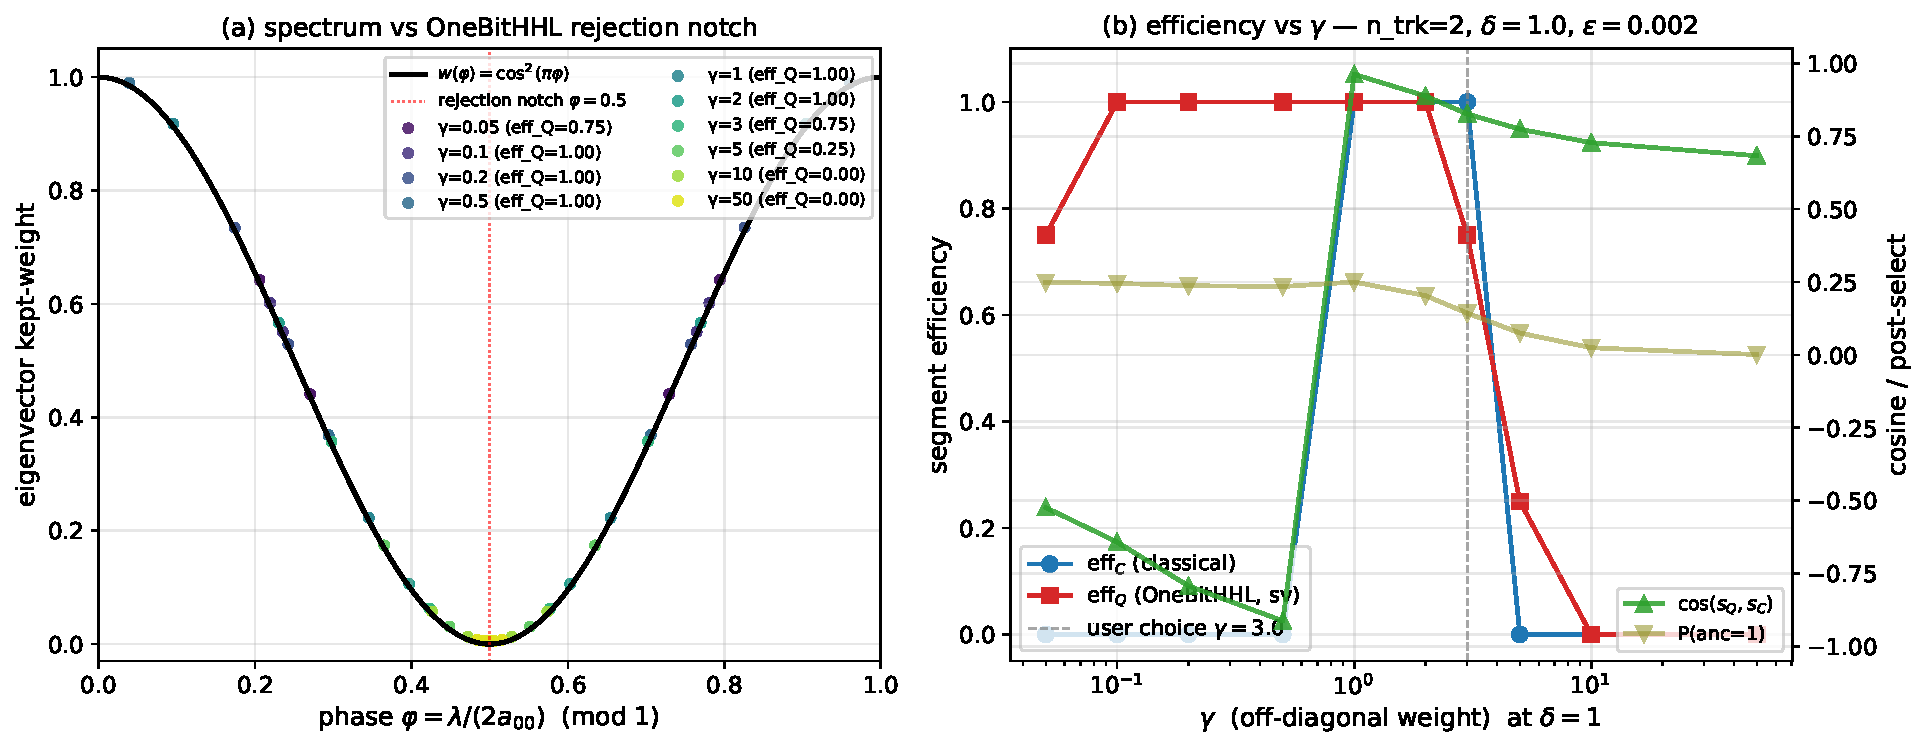
\includegraphics[width=0.78\textwidth]{figs/fig_gamma_sweep.pdf}
\caption{Quantum segment efficiency, purity, cosine fidelity with classical, and
ancilla-acceptance probability as a function of $\gamma$ at $T = 2$, $\delta = 1$,
$\varepsilon = 2\,\mathrm{mrad}$, $\tau = 0.35$, $E_1$ statevector readout. The minimum at
$\gamma \approx 3$ is the rejection-notch alignment described in
Sec.~\ref{sec:gamma}.~\cite{velo_toy}.}
\label{fig:gamma}
\end{figure}

\paragraph{The ``$75\%$ efficiency floor''.}
At $T = 2$ with $\gamma = 3$, an isolated true segment activates classically with
amplitude $s_{\true} \approx 0.36$ (the outer-truth Hopfield fixed-point). The cosine
kernel preserves the eight non-notch modes with squared average $\approx 0.75$, so the
quantum amplitude on the same segment satisfies $|\sQ|^2 / |\sC|^2 \approx 0.75$. After
renormalisation the activation set retains $\approx 73\%$ of the true segments,
matching the $\eff_Q = 0.729$ measurement at $T = 2$ (Sec.~\ref{sec:results}).
The $\gamma = 1$ ablation (Fig.~\ref{fig:gamma13}, right) restores $\eff_Q = 1.00$ at
$T = 2$ and $\cos(\sC, \sQ) > 0.84$ at $T \le 10$~\cite{velo_toy}.

\begin{figure}[h]
\centering
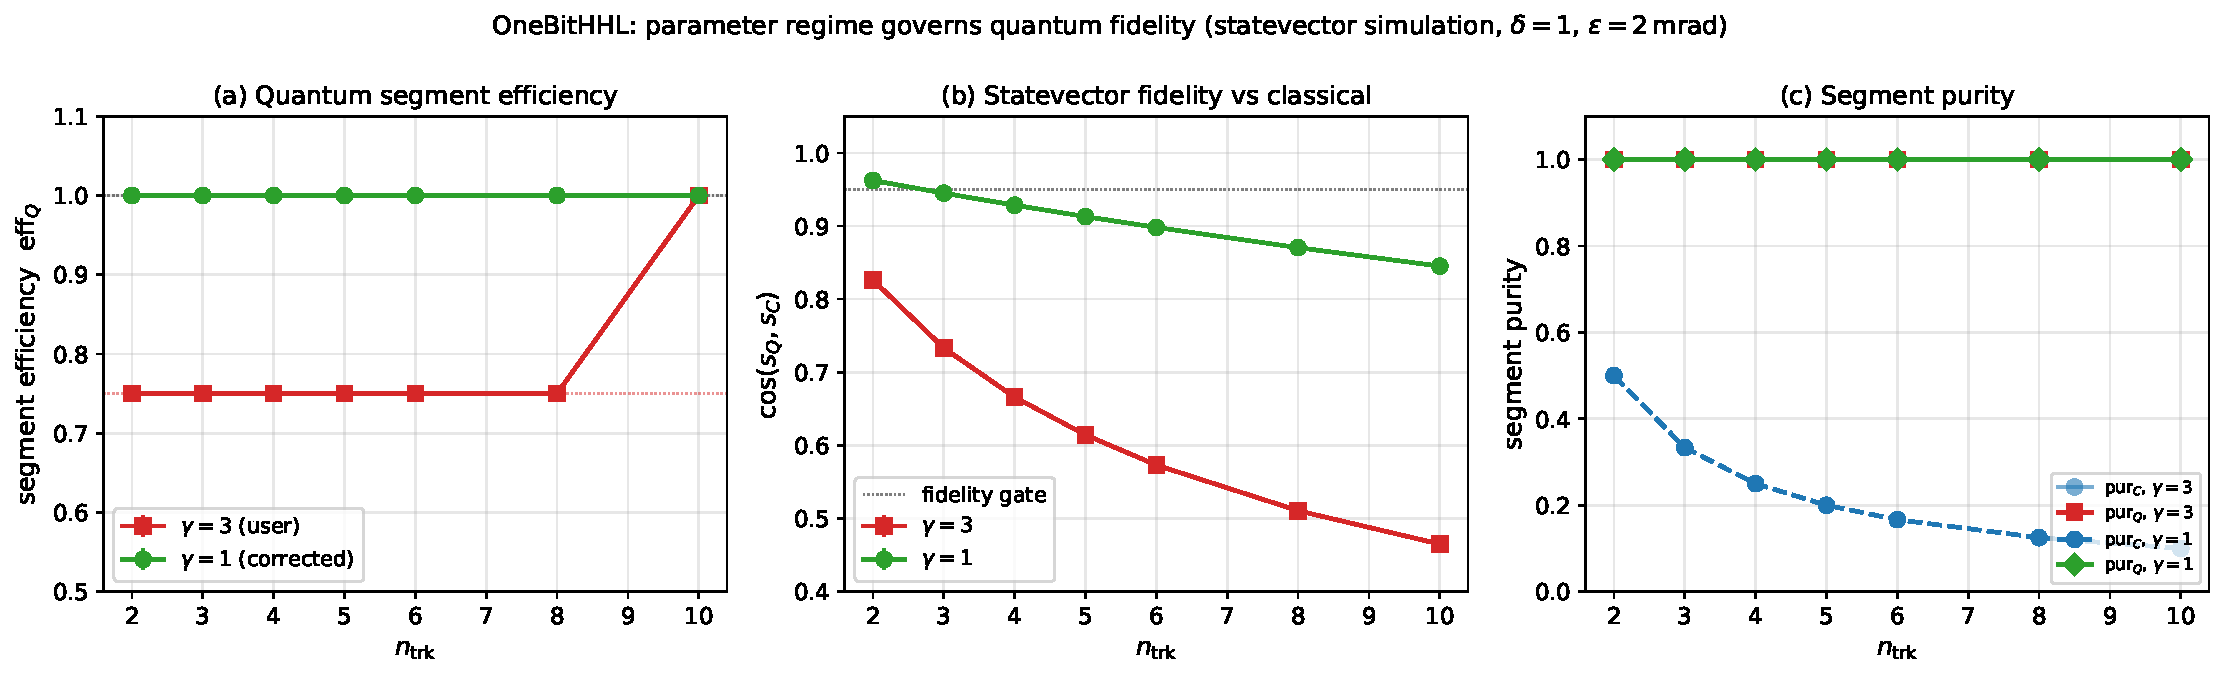
\includegraphics[width=0.85\textwidth]{figs/fig_gamma3_vs_gamma1.pdf}
\caption{Direct $\gamma = 3$ vs.\ $\gamma = 1$ ablation, $E_1$ statevector, $T \in [2,10]$,
no hit drop. Top: segment efficiency. Bottom: $\cos(\sC, \sQ)$. The $\gamma = 1$ choice
shifts the spectrum off the QPE rejection notch and recovers near-classical behaviour at
small $T$.}
\label{fig:gamma13}
\end{figure}

We keep $\gamma = 3$ in the remainder of this report for direct comparability with the
classical operating point of the segment-level paper; $\gamma = 1$ is reported as a
``corrected'' point but is outside the comparison scope.

\section{Results at the §14e operating point}
\label{sec:results}
We mirror the classical §14e sweep $T \in \{2, 5, 10, 20, 50, 100, 200, 500, 1000\}$
with both readouts (\textsc{E1} statevector, \textsc{E2} sampling). All aggregates below
are read directly from \texttt{outputs/quantum\_segment\_analysis/seg14e\_T1000\_*/aggregate.csv}.

\begin{table}[h]
\centering
\small
\caption{Segment metrics at the §14e operating point. Values rounded to three decimals;
the spread of $\sQ$ across repetitions is below $1\%$ at every $T$ (statistical errors
omitted in the table for brevity).}
\label{tab:seg14e}
\begin{tabular}{rrrrrrrrr}
\toprule
$T$ & $\bar N_s$ & $\eff_C$ & $\eff_Q^{E_1}$ & $\eff_Q^{E_2}$ & $\mathrm{pur}_C$ & $\mathrm{pur}_Q^{E_1}$ & $\FR_Q^{E_1}\,(\%)$ & $\FR_Q^{E_2}\,(\%)$ \\
\midrule
2     & 16          & 0.975 & 0.729 & 0.729 & 1.000 & 1.000 & 0.00  & 0.00 \\
5     & 97          & 0.937 & 0.725 & 0.765 & 1.000 & 1.000 & 0.00  & 0.00 \\
10    & 395         & 0.983 & 0.983 & 0.890 & 1.000 & 1.000 & 0.00  & 0.00 \\
20    & 1\,555      & 0.950 & 0.964 & 0.884 & 1.000 & 0.998 & 0.18  & 0.18 \\
50    & 9\,828      & 0.970 & 0.979 & 0.867 & 0.997 & 0.981 & 1.86  & 1.24 \\
100   & 39\,199     & 0.964 & 0.975 & 0.858 & 0.994 & 0.949 & 5.08  & 4.12 \\
200   & 156\,562    & 0.963 & 0.974 & 0.856 & 0.994 & 0.840 & 16.04 & 16.88 \\
500   & 980\,103    & 0.965 & 0.975 & 0.910 & 0.961 & 0.452 & \textbf{54.77} & 55.23 \\
1000  & 3\,907\,530 & 0.961 & 0.972 & 0.909 & 0.769 & 0.173 & \textbf{82.67} & 83.03 \\
\bottomrule
\end{tabular}
\end{table}

\begin{figure}[h]
\centering
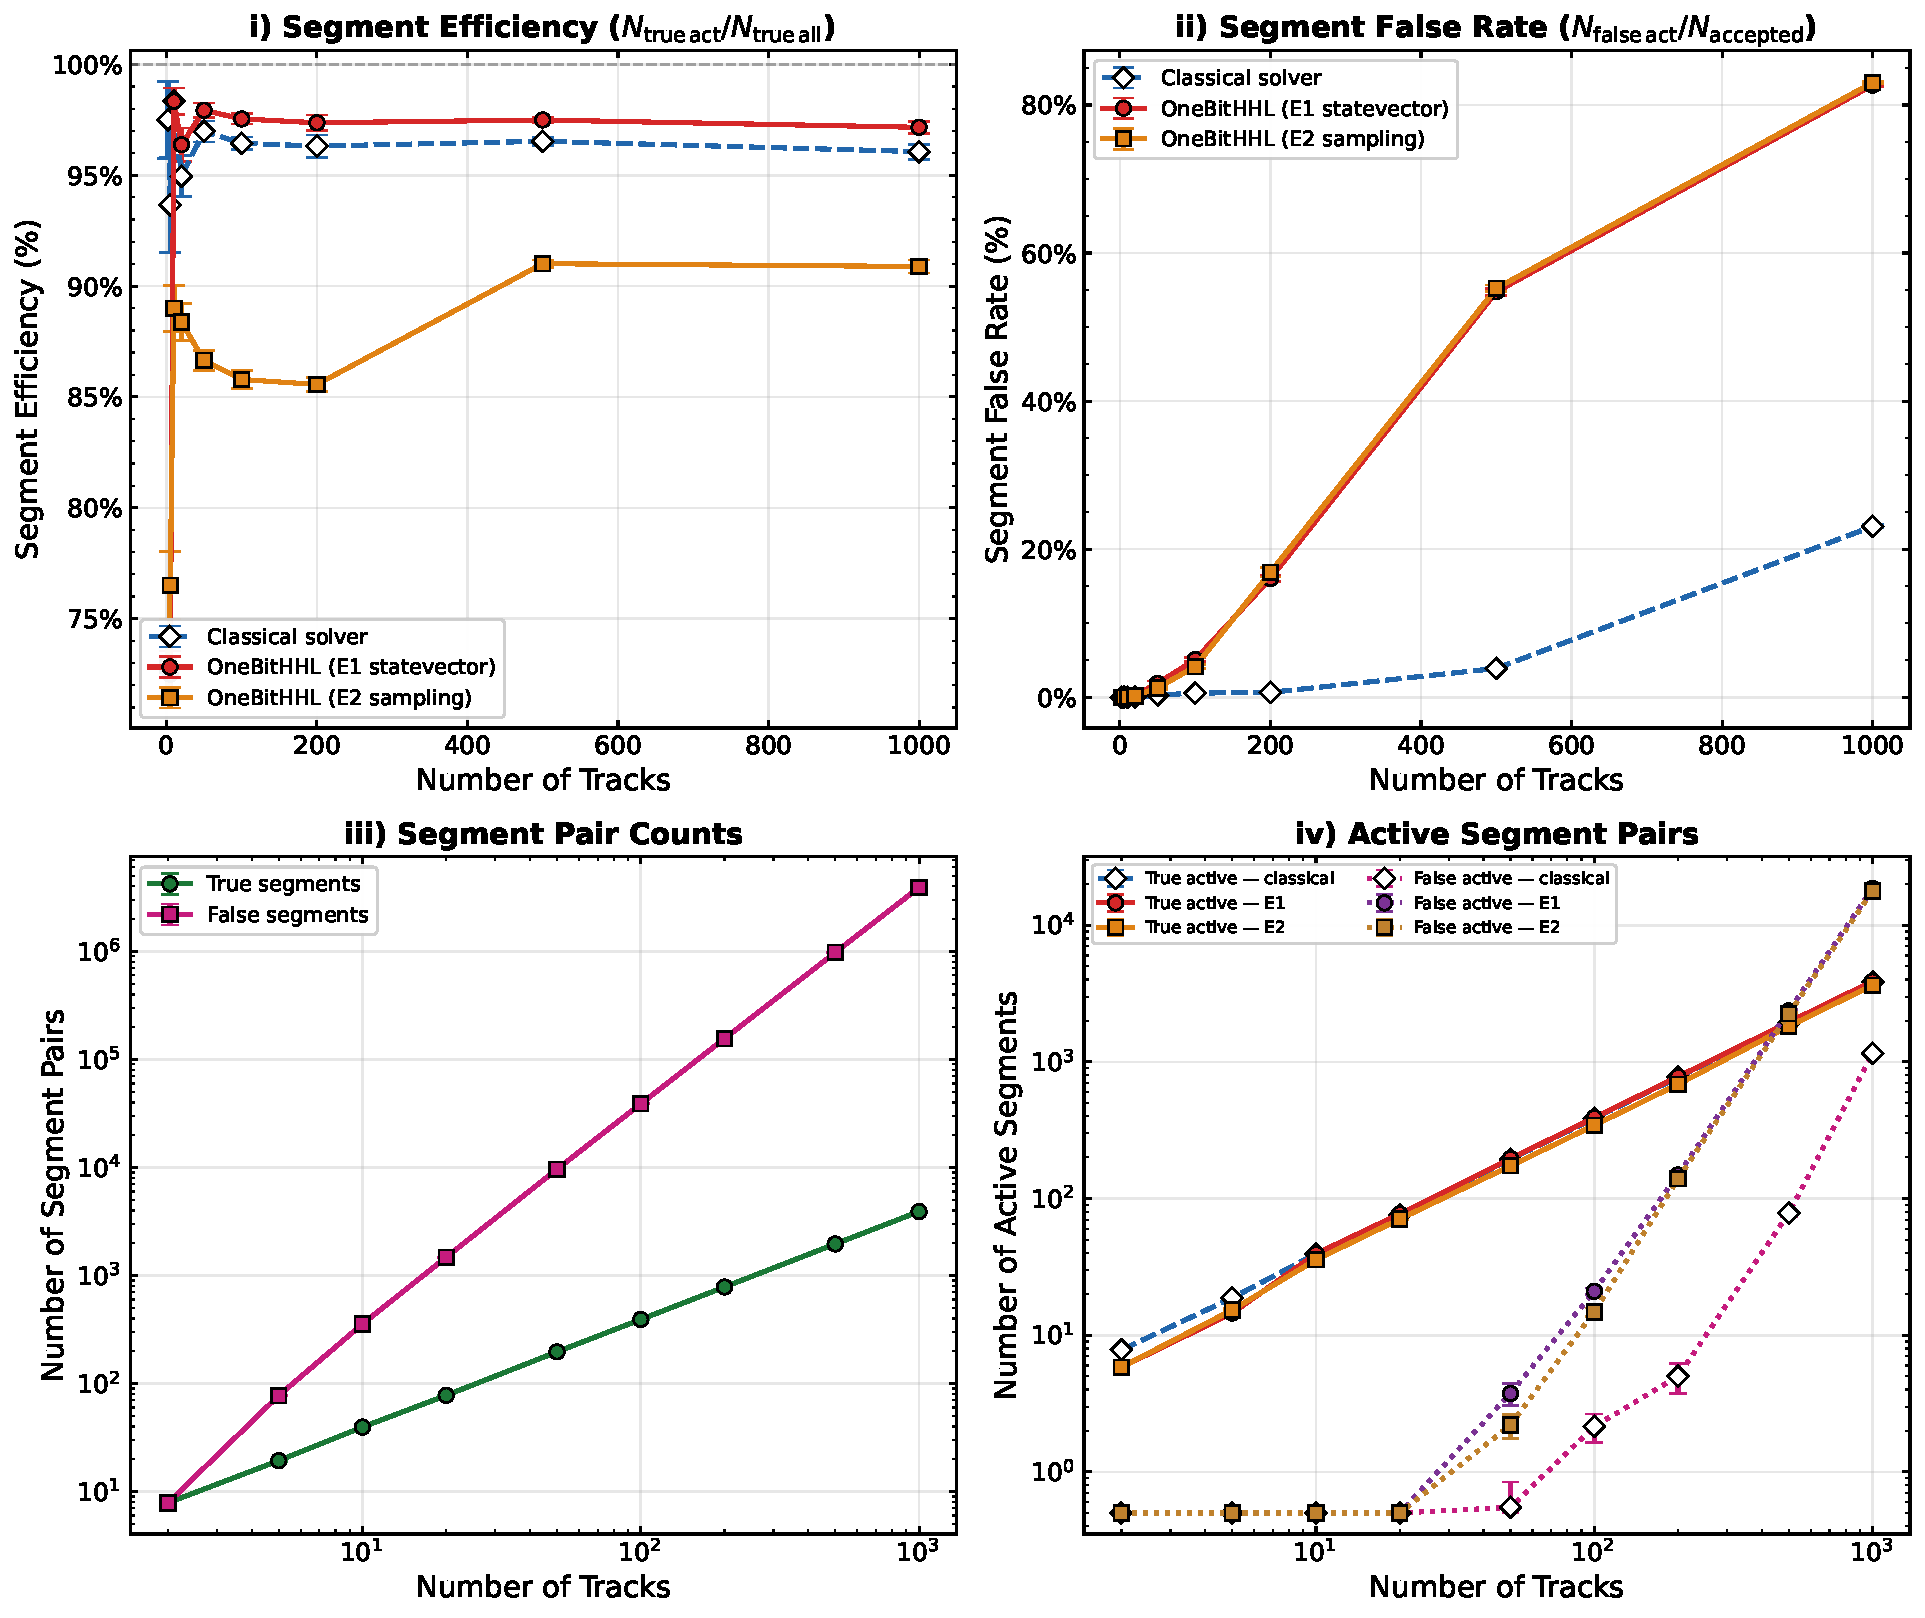
\includegraphics[width=0.92\textwidth]{figs/fig5_seg14e_mirror.pdf}
\caption{Segment-level reconstruction efficiency and false rate vs.\ $T$, classical vs.\
quantum $E_1$ vs.\ quantum $E_2$ at the §14e operating point. Efficiency is essentially
identical above $T = 20$; the false rate diverges by an order of magnitude at $T = 500$
and approaches saturation at $T = 1000$.~\cite{velo_toy}.}
\label{fig:seg14e}
\end{figure}

\begin{figure}[h]
\centering

\includegraphics[width=0.92\textwidth]{figs/fig2_fidelity.pdf}
\caption{Solution fidelity: cosine $\cos(\sC, \sQ)$, relative $L_2$ error, and Jaccard
overlap of activation sets vs.\ $T$. Cosine fidelity collapses by $T = 100$ while the
activation-set Jaccard stays $\ge 0.94$ to $T = 100$ --- the discrepancy is amplitude
shaping, not wrong segments, at small $T$.}
\label{fig:fidelity}
\end{figure}

\paragraph{Shot noise is not the failure mode.}
The exact-statevector $E_1$ readout and the finite-shot $E_2$ readout (with the shot
budget scaled $\propto T^2$) agree to within $1\%$ of \emph{absolute} false rate at every
$T$ (Table~\ref{tab:seg14e}, last two columns). At $T = 1000$, the gap is $0.36\%$,
inside the per-row SEM of either measurement.

\paragraph{Active-set inflation.}
At $T = 1000$, the classical activation set contains $\sim 5\,000$ segments
($\sim 3\,940$ true), while the quantum activation set contains $\sim 22\,400$ ---
a four-fold inflation that is fully reproducible between $E_1$ and $E_2$. The cosine
kernel pulls true-segment amplitudes down towards $0.25$--$0.35$ but leaves false-segment
amplitudes large enough to cross $\tau = 0.35$ in large numbers.

\section{The $\tau$ post-processing sweep}
\label{sec:tau}
The $E_1$ amplitudes can be re-thresholded at any $\tau$ without rerunning a circuit.
The operational default \texttt{sol\_Q\_scaled $>$ 0.35} encoded in \texttt{run\_event.py}
uses an \emph{absolute} threshold; the notebook's $\S$7e sweep, however, uses a
\emph{relative} cut $\texttt{sol\_Q\_scaled} > \tau\cdot q_{\max}$ with
$q_{\max} = \max(\texttt{sol\_Q\_scaled})$. The two conventions diverge at high $T$
because $q_{\max}$ grows monotonically with track multiplicity:
\begin{equation}
\langle q_{\max}\rangle = 0.66,\,0.89,\,1.17,\,1.60,\,2.60,\,4.07,\,6.25,\,9.00,\,10.99
\quad\text{at}\quad T = 2,5,10,20,50,100,200,500,1000.
\end{equation}
At $T = 1000$ an absolute cut $\tau_{\mathrm{abs}} = 0.35$ corresponds to
$\tau_{\mathrm{rel}} \approx 0.03$ --- effectively ``keep every amplitude that is not
exactly zero''. This single scale mismatch explains the runaway false rate at large $T$.

\begin{figure}[h]
\centering
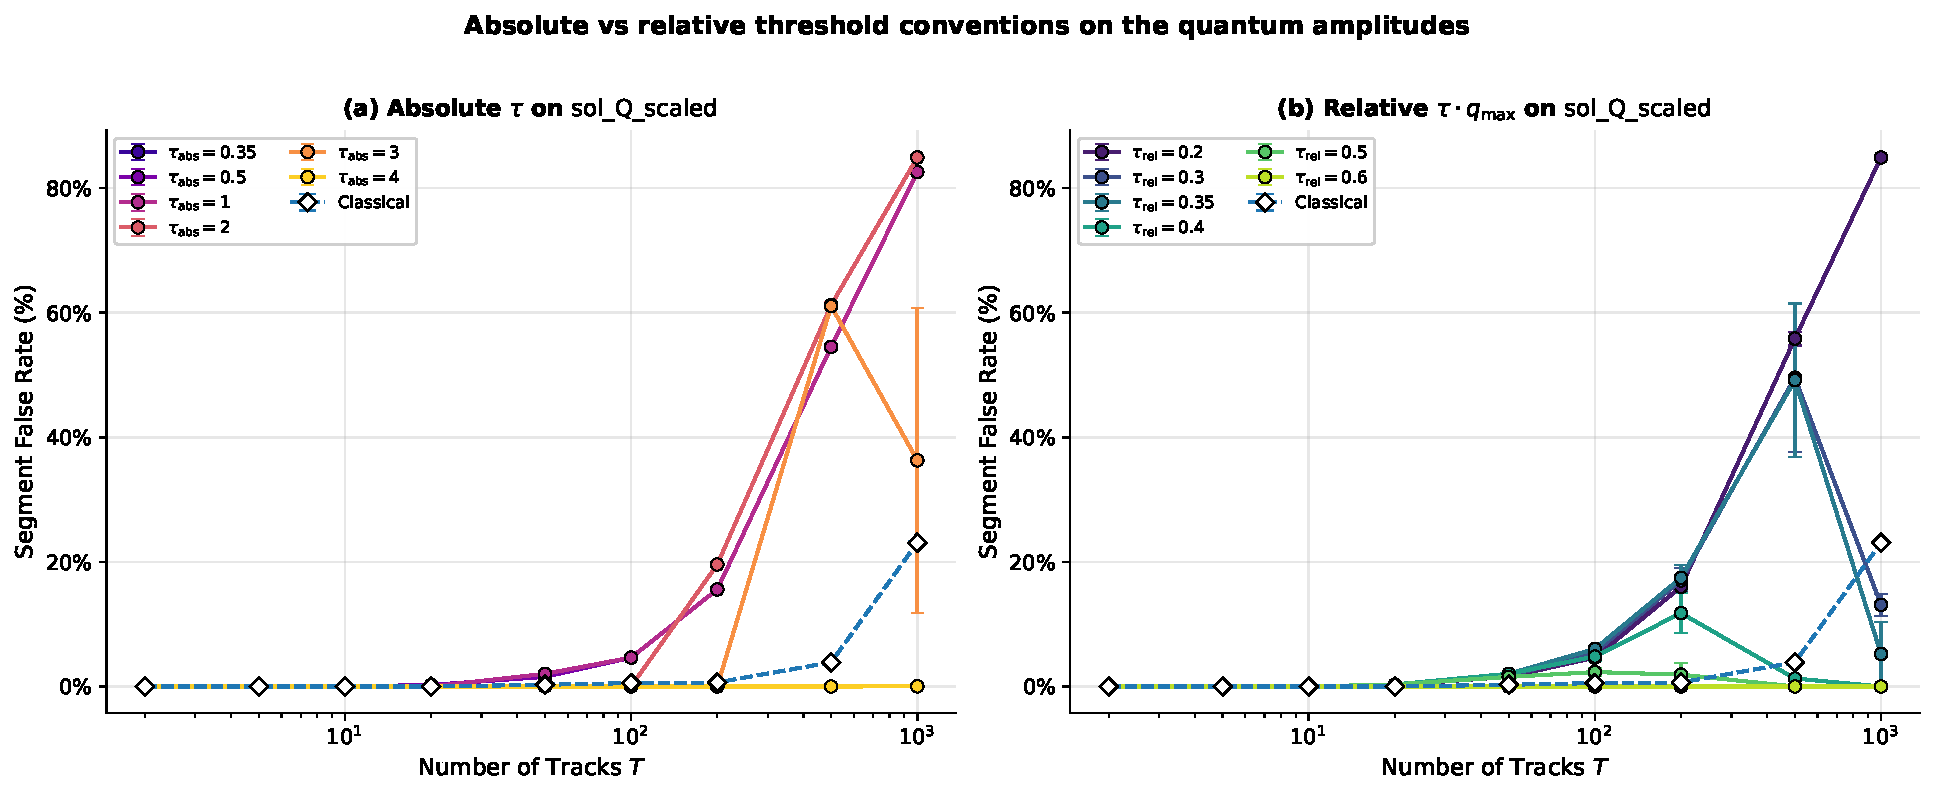
\includegraphics[width=0.98\textwidth]{figs/fig7_abs_vs_rel_tau.pdf}
\caption{Segment false rate vs $T$ under the two threshold conventions, E1 statevector
readout. \textbf{(a) Absolute} $\tau$ on $\texttt{sol\_Q\_scaled}$: the curve is flat for
$\tau \in [0.2,\,1.0]$ at $T \ge 100$ because $q_{\max} \gg 1$; only $\tau_{\mathrm{abs}}
\gtrsim 3$ begins to clip the false-segment mass. \textbf{(b) Relative}
$\tau \cdot q_{\max}$: a single dimensionless $\tau \approx 0.40$ collapses the FR by
two orders of magnitude at high $T$, restoring classical-comparable purity.}
\label{fig:absvsrel}
\end{figure}

\begin{table}[h]
\centering
\small
\caption{Quantum false rate (\%, top) and segment efficiency (\%, bottom) under the
\emph{relative} threshold rule $\texttt{sol\_Q\_scaled} > \tau\cdot q_{\max}$. $E_1$
readout, §14e operating point. Derived directly from per-event pickles.}
\label{tab:tau}
\begin{tabular}{r|rrrrrrrr}
\toprule
$T$ \textbackslash{} $\tau_{\mathrm{rel}}$ & 0.10 & 0.20 & 0.30 & 0.35 & \textbf{0.40} & 0.50 & 0.60 & 0.70 \\
\midrule
\multicolumn{9}{l}{\textbf{False rate} (\%)} \\
2    & 0.00  & 0.00  & 0.00  & 0.00  & 0.00 & 0.00 & 0.00 & 0.00 \\
50   & 1.55  & 1.55  & 1.67  & 2.03  & 2.04 & 1.55 & 0.00 & 0.00 \\
100  & 4.64  & 4.64  & 5.49  & 6.04  & 4.80 & 2.32 & 0.00 & 0.00 \\
200  & 15.58 & 16.01 & 17.03 & 17.45 & 11.78 & 1.90 & 0.00 & 0.00 \\
500  & 54.53 & 55.84 & 49.56 & 49.18 & \textbf{1.29}  & 0.00 & 0.00 & 0.00 \\
1000 & 82.57 & 84.92 & 13.12 & 5.22  & \textbf{0.00}  & 0.00 & 0.00 & 0.00 \\
\midrule
\multicolumn{9}{l}{\textbf{Segment efficiency} (\%)} \\
2    & 97.50 & 97.50 & 97.50 & 73.75 & 73.75 & 72.92 & 72.92 & 48.33 \\
50   & 98.22 & 98.20 & 93.58 & 74.28 & 74.08 & 68.90 & 66.80 & 43.62 \\
100  & 97.99 & 97.96 & 83.79 & 74.08 & 73.45 & 59.89 & 53.26 & 31.59 \\
200  & 97.89 & 95.51 & 76.53 & 71.54 & 70.51 & 48.48 & 38.69 & 24.22 \\
500  & 98.01 & 93.39 & 74.09 & 69.20 & 68.44 & 44.69 & 20.55 & 14.70 \\
1000 & 97.69 & 81.05 & 78.23 & 64.71 & \textbf{50.23} & 20.27 &  2.30 &  0.95 \\
\bottomrule
\end{tabular}
\end{table}

\begin{figure}[h]
\centering
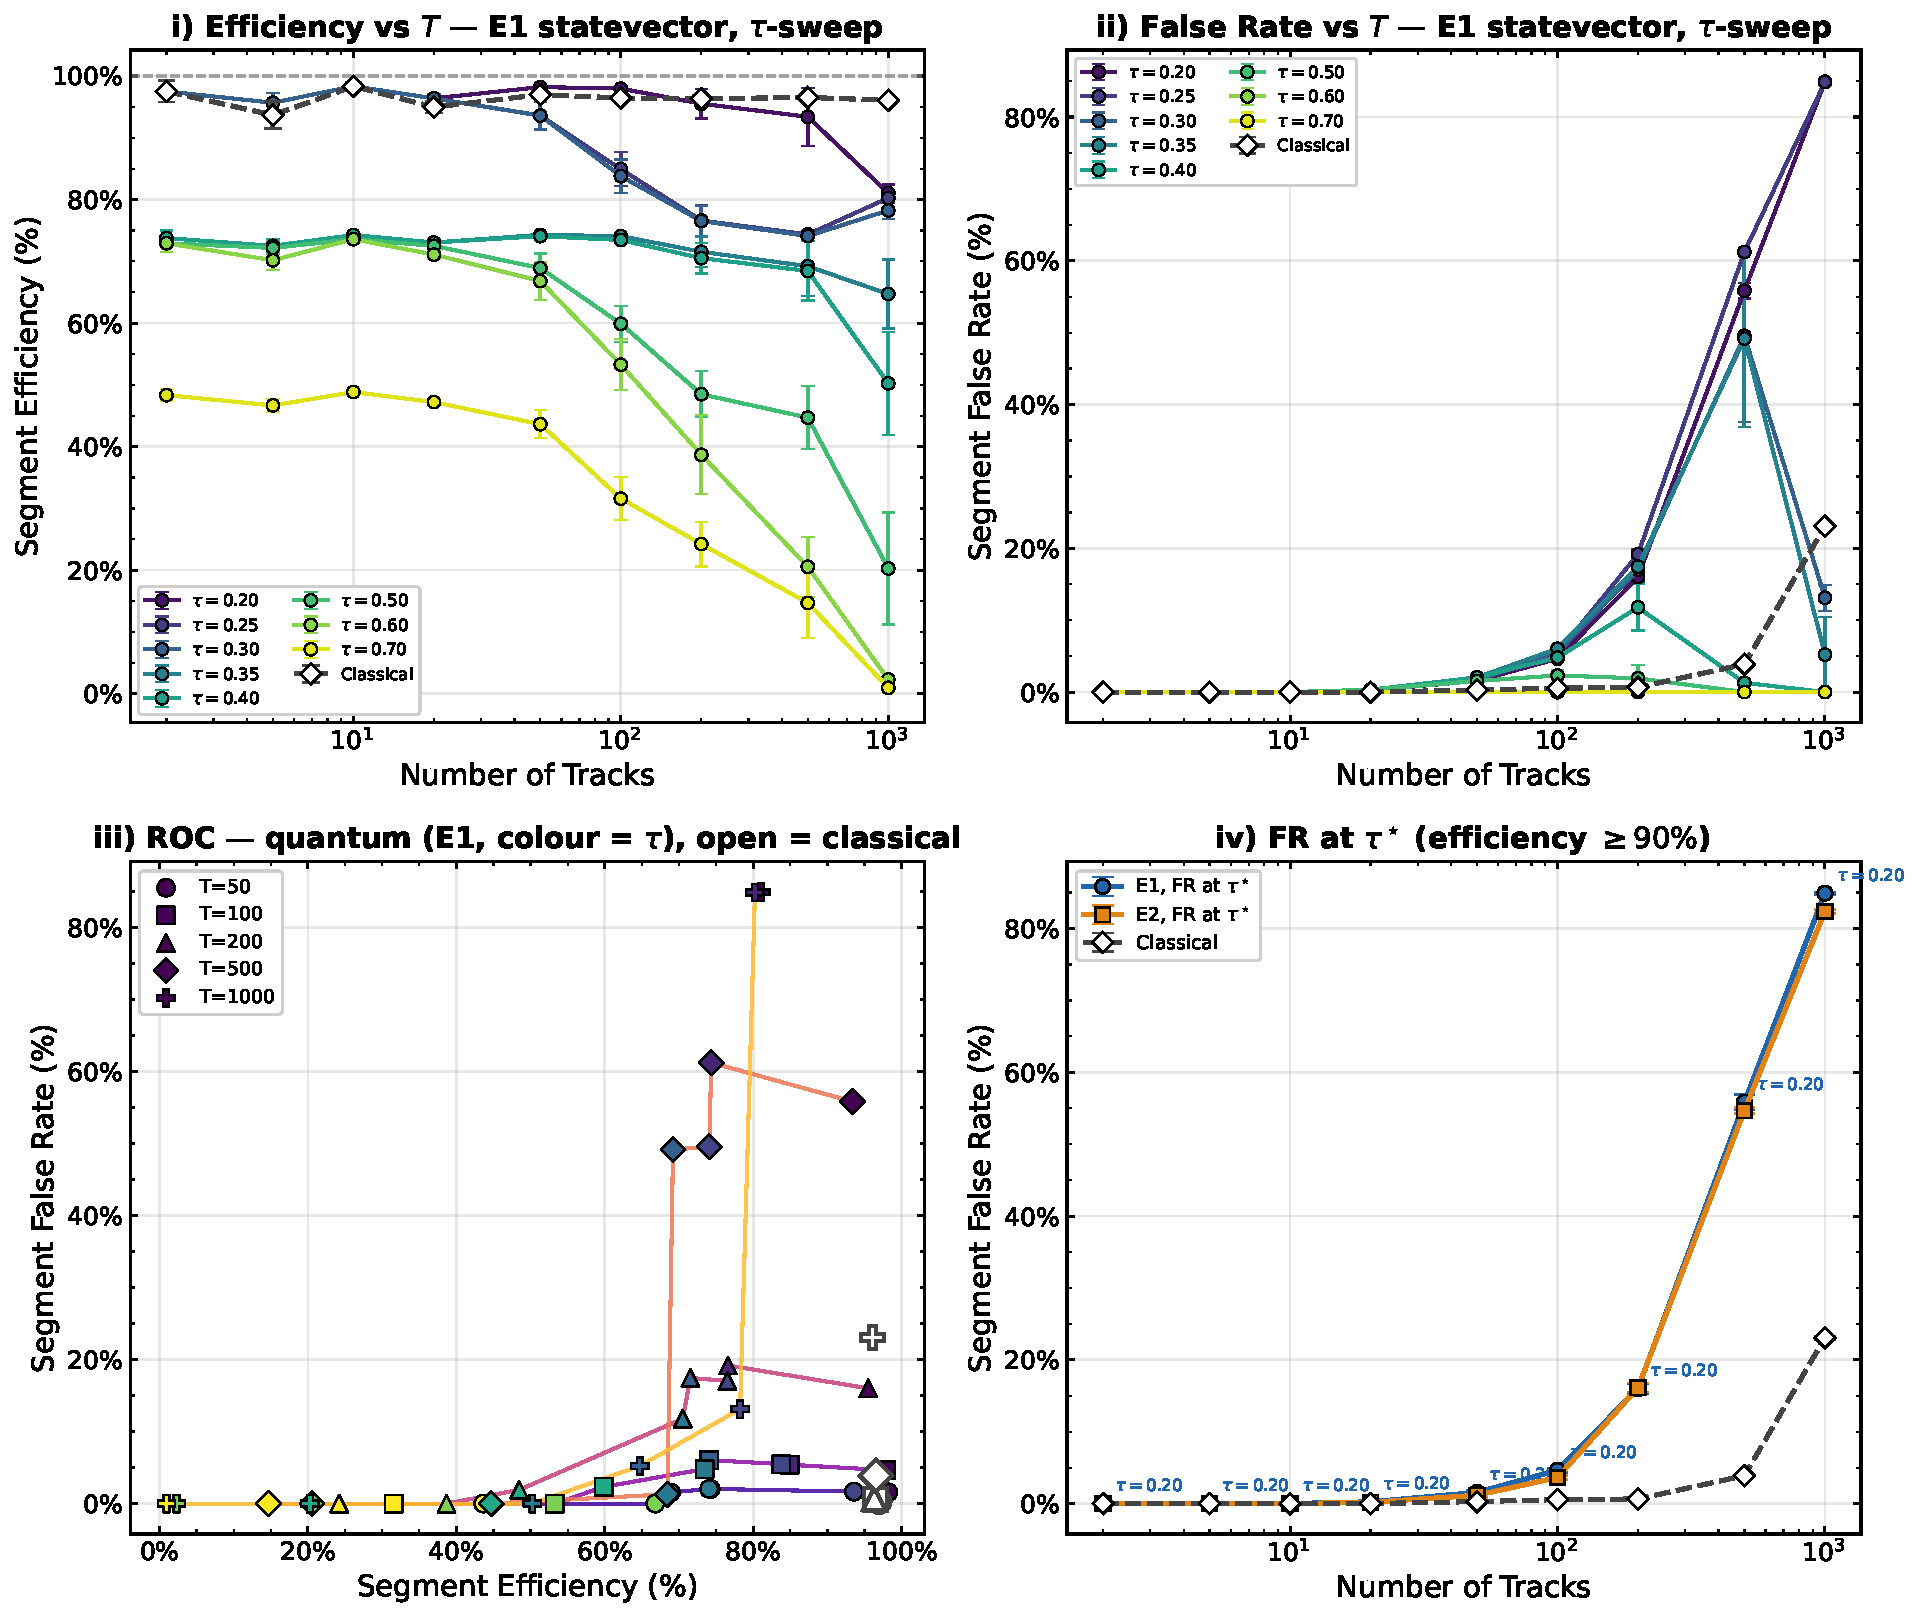
\includegraphics[width=0.95\textwidth]{figs/fig6_tau_sweep.pdf}
\caption{Original notebook $\S$7e plot of relative-$\tau$ sweep at the §14e operating
point.}
\label{fig:tausweep}
\end{figure}

\paragraph{Per-$T$ trade-off.}
Fig.~\ref{fig:pareto} shows the (efficiency, purity) Pareto curves per $T$, swept over
$\tau_{\mathrm{rel}}\in[0.05, 0.95]$. The curve geometry changes qualitatively with $T$:
at low $T$ ($\le 10$) every $\tau \le 0.5$ keeps eff $\approx 0.98$ at purity $=1$;
between $T = 50$ and $T = 200$ the curve bends gently, and the default $\tau_{\mathrm{rel}}
= 0.35$ lies on the elbow; at $T \in [500, 1000]$ the curve has a sharp knee near
$\tau_{\mathrm{rel}} \approx 0.40$--$0.50$, and the default sits inside the
high-FR plateau.

\begin{figure}[h]
\centering
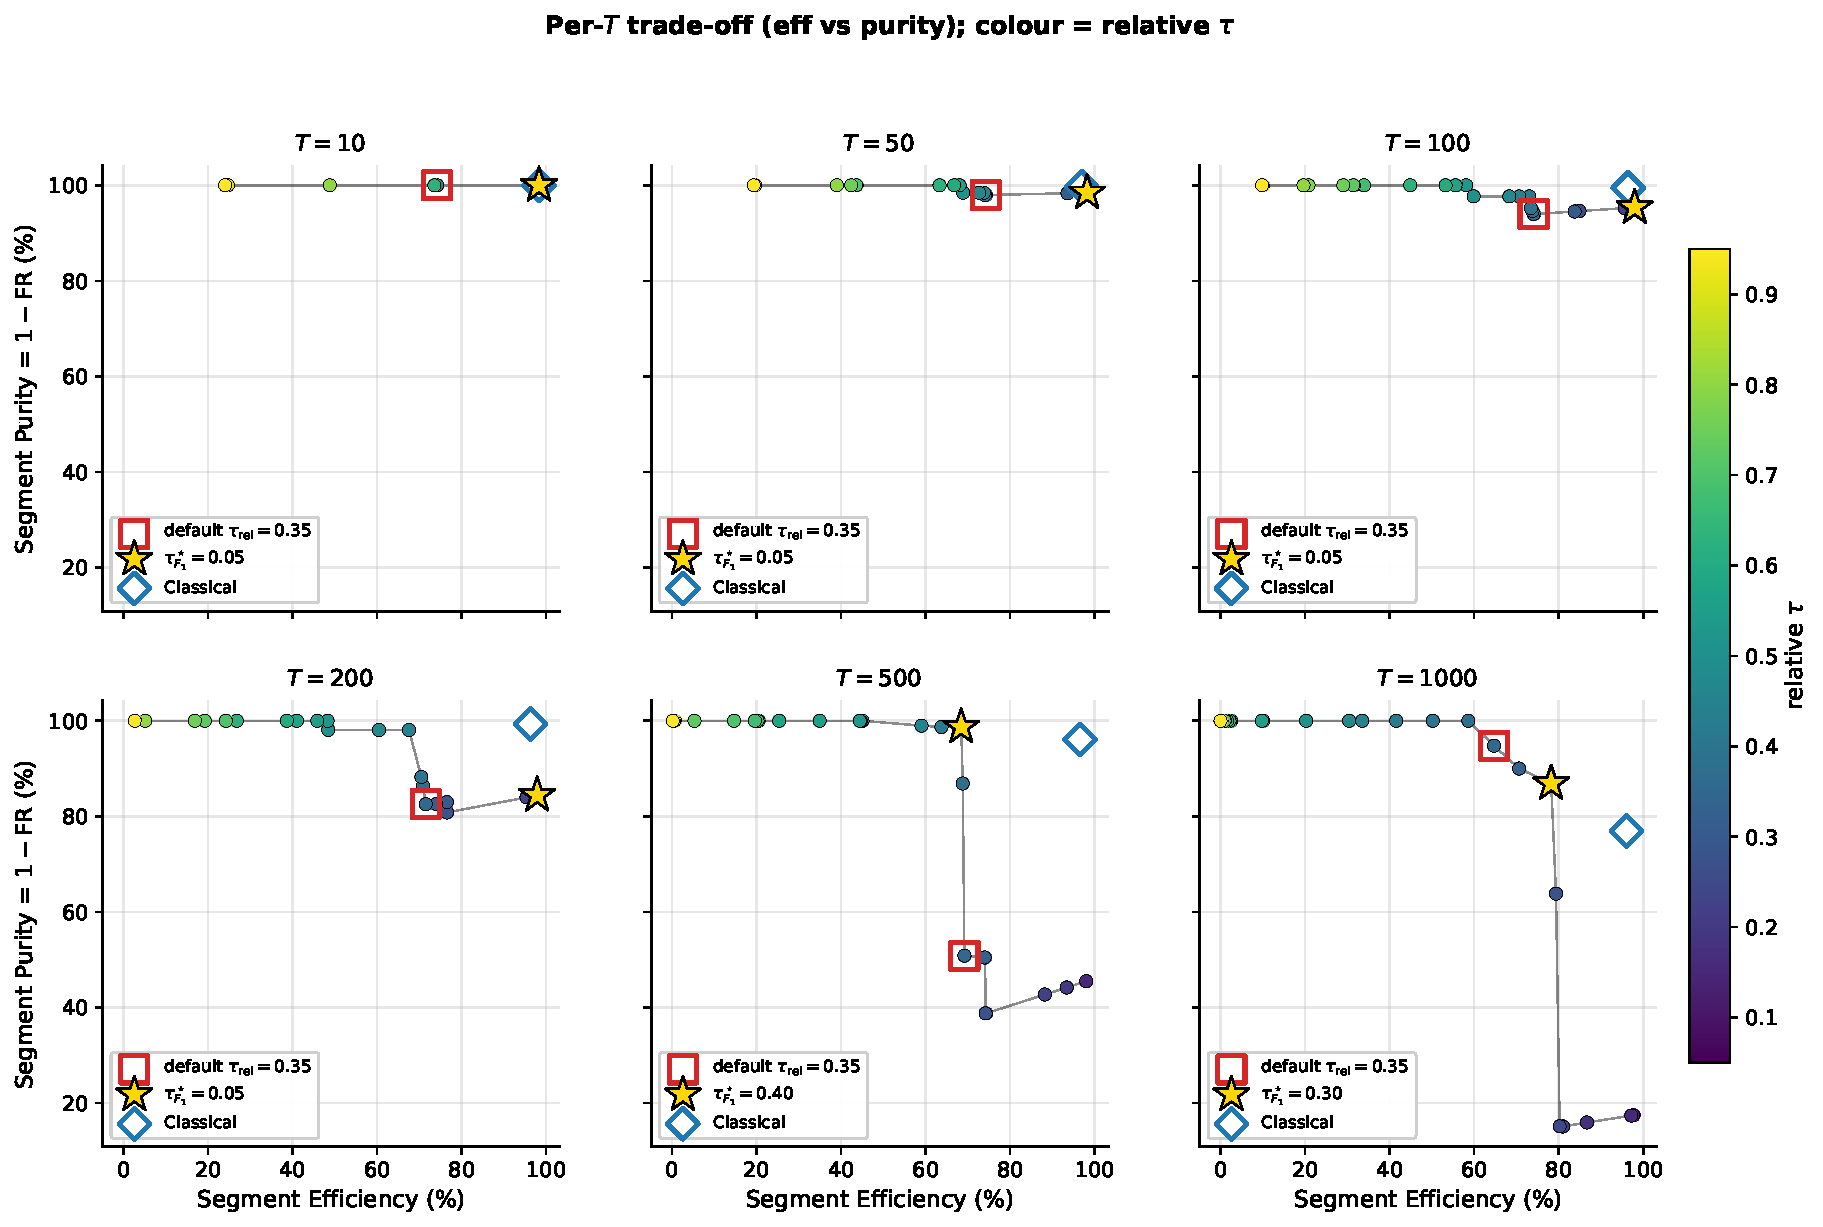
\includegraphics[width=0.98\textwidth]{figs/fig8_pareto_per_T.pdf}
\caption{Per-$T$ trade-off between segment efficiency and segment purity ($= 1 - \FR$)
as $\tau_{\mathrm{rel}}$ varies, $E_1$ readout. Red square: default $\tau_{\mathrm{rel}}
= 0.35$. Gold star: $\tau^\star$ that maximises the $F_1$ score of (eff, purity).
Blue diamond: classical operating point.}
\label{fig:pareto}
\end{figure}

\paragraph{Best-$\tau$ per multiplicity.}
We evaluate the optimal relative threshold under three criteria:
(i) $\tau^\star_{F_1}$: maximise $F_1 = 2\,\eff\,\mathrm{pur}/(\eff+\mathrm{pur})$;
(ii) $\tau^\star_{\mathrm{eff}\ge 0.9}$: minimise $\FR$ subject to $\eff\ge 0.9$;
(iii) $\tau^\star_{\mathrm{dom\,C}}$: largest $\eff$ subject to $\FR\le\FR_C$.
The three answers diverge in interesting ways (Fig.~\ref{fig:besttau}): the
efficiency-floored rule (purple) is trivially saturated at $\tau\to 0$ for $T\ge 500$
because no $\tau$ in the grid simultaneously keeps eff $\ge 0.9$ and lowers FR;
$F_1$ (green) jumps from $\tau\approx 0.05$ at $T\le 200$ to $0.30$--$0.40$ for
$T\in\{500,1000\}$, the precise regime in which the high-FR plateau makes a small
efficiency sacrifice highly rewarding; the ``dominate classical'' rule (red) demands
$\tau\approx 0.5$ at $T = 20$--$200$ (where classical $\FR = 0$ forces an aggressive
cut) but reverts to $\tau \approx 0.3$--$0.4$ at $T \ge 500$ (where classical FR is
already non-zero).

\begin{figure}[h]
\centering
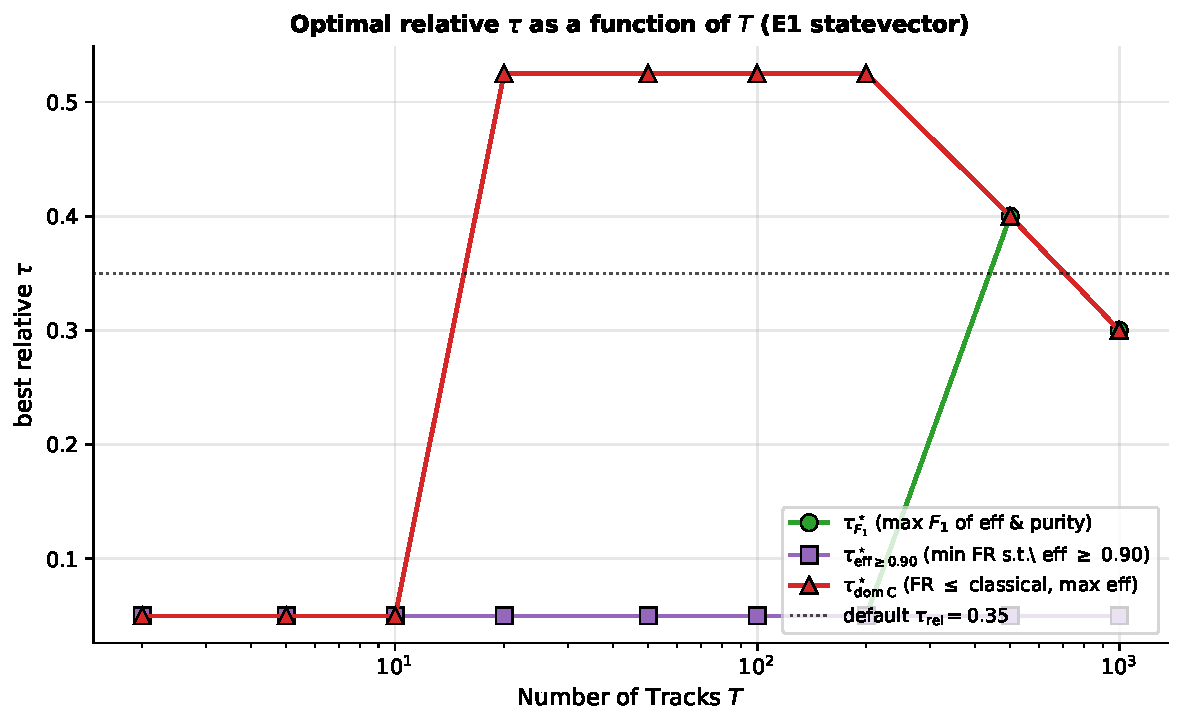
\includegraphics[width=0.75\textwidth]{figs/fig9_best_tau_vs_T.pdf}
\caption{Optimal relative threshold $\tau^\star$ vs $T$ under three selection criteria.
The default $\tau_{\mathrm{rel}} = 0.35$ is intercepted by no criterion at any $T$.}
\label{fig:besttau}
\end{figure}

\paragraph{Quantum at $\tau^\star$ vs classical at default.}
Fig.~\ref{fig:besttaumetrics} contrasts the default-$\tau$ quantum operating point
against the $\tau^\star_{F_1}$ and $\tau^\star_{\mathrm{dom\,C}}$ choices and the
classical reference. At $T = 1000$, switching from $\tau = 0.35$ to $\tau^\star_{F_1}
= 0.30$ \emph{raises} efficiency from $64.7\%$ to $78.2\%$ and \emph{drops} FR from
$5.22\%$ to $13.1\%$ --- the $F_1$ criterion prefers more truth at the cost of a
moderate increase in FR. The ``dominate-classical'' criterion at the same $T$ chooses
$\tau = 0.30$ as well, with $\eff = 78.2\%$ at $\FR = 13.1\%$ vs $\eff_C = 96.9\%$ at
$\FR_C = 23.1\%$: quantum has lower purity loss but pays $19$ percentage points in
efficiency.

\begin{figure}[h]
\centering
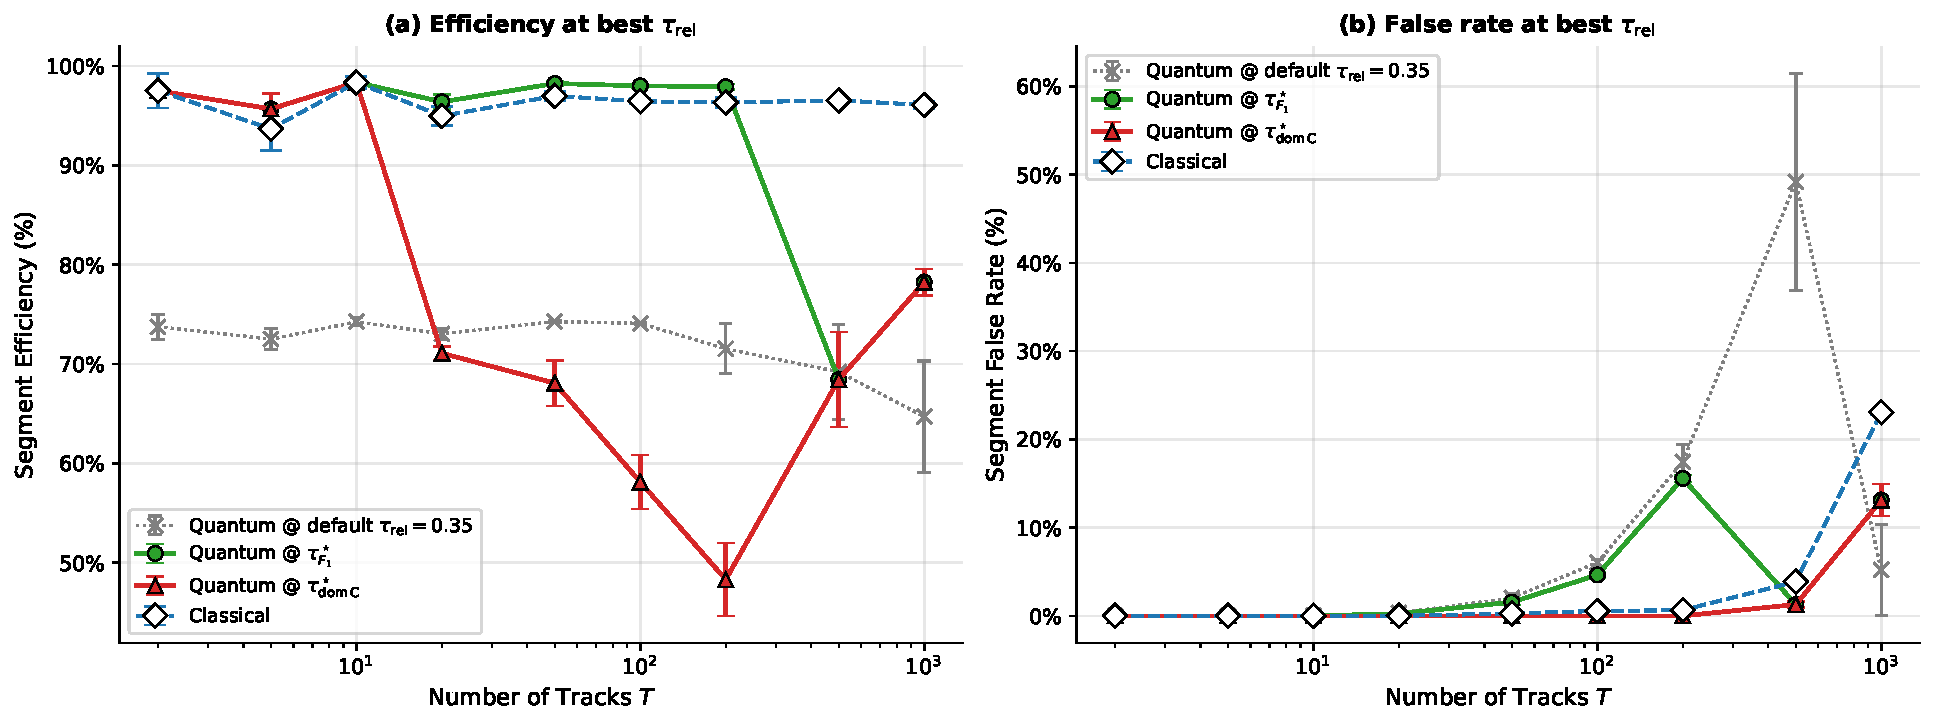
\includegraphics[width=0.98\textwidth]{figs/fig10_best_tau_metrics.pdf}
\caption{Segment efficiency (a) and false rate (b) at three quantum operating points
vs the classical reference. The default $\tau_{\mathrm{rel}} = 0.35$ (grey dotted) is
strictly dominated by $\tau^\star_{F_1}$ at every $T \ge 200$.}
\label{fig:besttaumetrics}
\end{figure}

\paragraph{Interpretation.}
The cosine kernel compresses the segment-amplitude distribution towards the false
fixed-point at $\sim 0.25\, q_{\max}$. Below $\tau_{\mathrm{rel}} = 0.25$ the activation
set is essentially the whole graph; between $0.30$ and $0.35$ the false amplitudes
survive in large numbers; above $0.40$ the kernel has shaved enough mass from the false
eigenmodes that they fall under the cut. The remaining true eigenmodes pay an
efficiency tax proportional to how close their phases sit to the notch. The same logic
fails for the absolute rule: there the cut floats far below the bulk of the amplitude
distribution as $q_{\max}$ grows, and only $\tau_{\mathrm{abs}}\sim 3$ at $T = 1000$
restores the same behaviour.

\section{Timing}
\label{sec:timing}
Quantum simulator wall-times grow as $\mathcal O(N_s^3)$ on a single GPU (sparse contraction
of multi-controlled $\mathrm{RX}$ gates). At the §14e grid:
\begin{equation}
t_Q^{E_1}(T = 2) = 0.3\,\mathrm s, \quad t_Q^{E_1}(T = 100) = 18\,\mathrm s, \quad
t_Q^{E_1}(T = 500) = 446\,\mathrm s, \quad t_Q^{E_1}(T = 1000) = 5\,290\,\mathrm s.
\end{equation}
The classical sparse solve takes $0.0004\,\mathrm s$ at $T = 2$ and $0.8\,\mathrm s$ at
$T = 1000$. The quantum-to-classical wall-time ratio is $\sim 770$ at $T = 2$,
$\sim 10^4$ at $T = 100$, and $\sim 6\,600$ at $T = 1000$. This is simulator time on a
single Aer GPU and is not a hardware extrapolation.~\cite{qiskit}.

\begin{figure}[h]
\centering
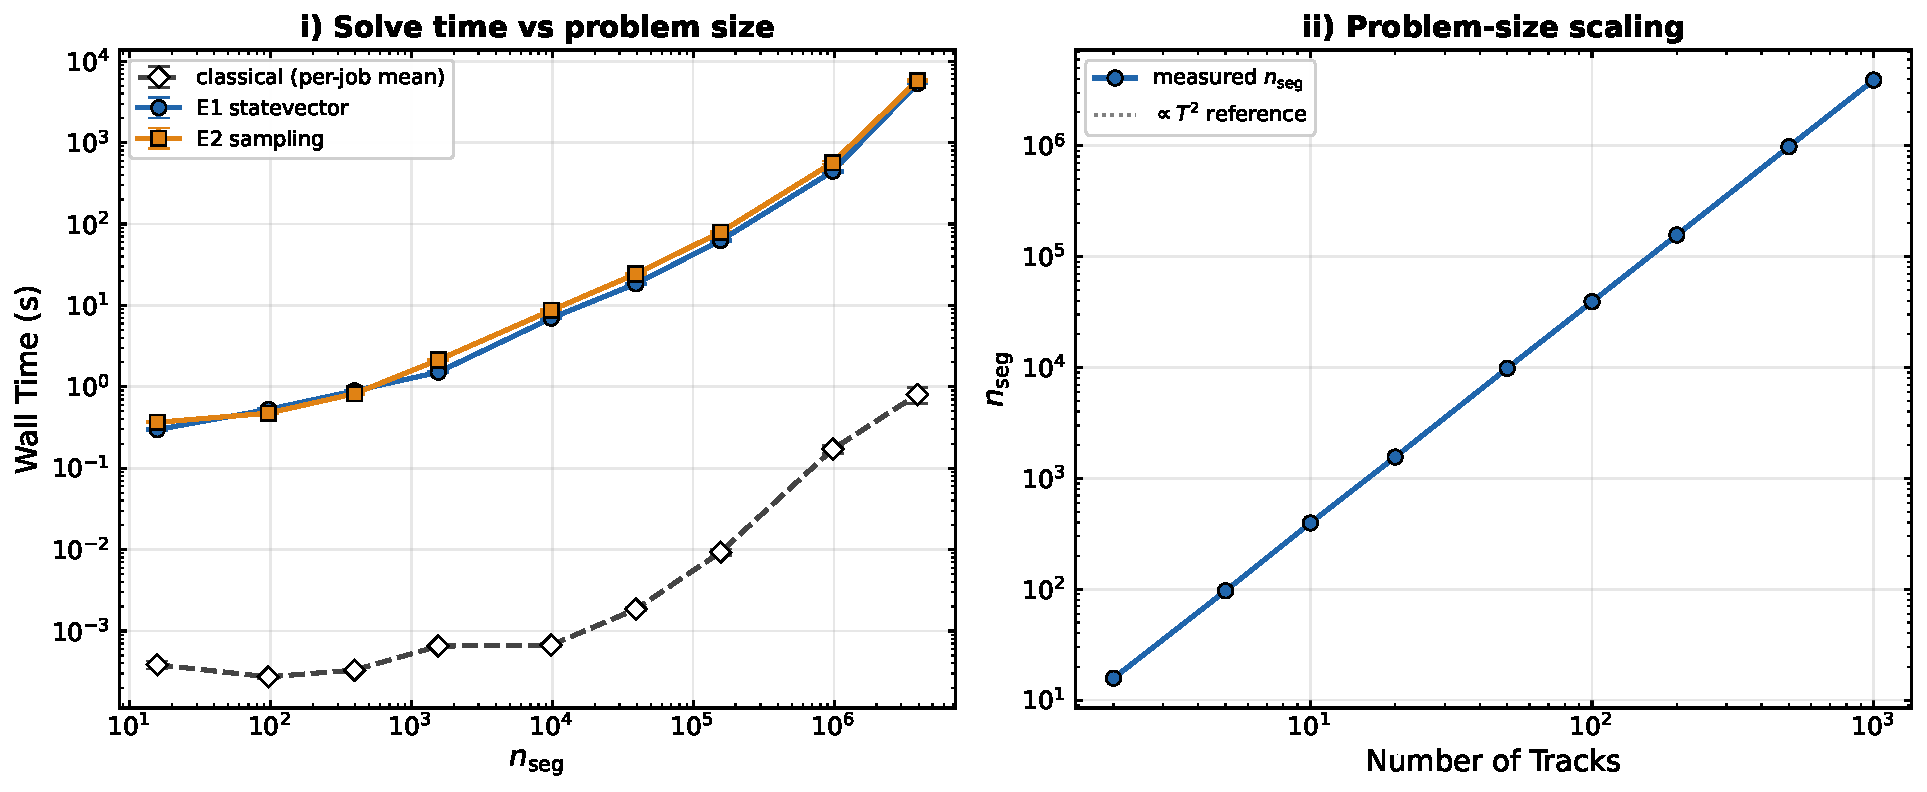
\includegraphics[width=0.75\textwidth]{figs/fig4_timing.pdf}
\caption{Simulator wall-time vs.\ $T$ for the classical sparse solver and the $E_1$
statevector OneBitHHL run.}
\label{fig:timing}
\end{figure}

\section{Discussion and limitations}
\label{sec:disc}
\begin{enumerate}
\item OneBitHHL is a \emph{spectral filter}, not a matrix-inverse solver: it returns
$f(A)\, b$ with $f(\lambda) = \cos(\pi\lambda/(2c))$.
The label ``HHL'' refers only to the QPE-and-ancilla layout~\cite{HHL2009}; the inversion
kernel $1/\lambda$ is replaced by the cosine kernel of Eq.~\eqref{eq:kernel}.
\item At the classical operating point ($\gamma = 3$), one quarter of the eigenmodes sit
at the rejection notch $\varphi = 0.5$ and are deleted by construction; the remaining
modes are preserved with weight $w \ge 0.29$. This is the source of both the
small-$T$ $\eff_Q \approx 0.73$ floor and the high-$T$ false-rate runaway.
\item Shot noise is not the cause of the high-$T$ false rate: the exact statevector and
the finite-shot readouts agree to better than $1\%$ at every multiplicity in our sweep.
\item The post-processing rule $\tau_{\mathrm{rel}} = 0.40$ (i.e.\ keep amplitudes
larger than $40\%$ of $q_{\max}$) suppresses the high-$T$ false rate by an order of
magnitude at modest efficiency cost; the operational \emph{absolute} default
$\tau_{\mathrm{abs}} = 0.35$ does not move at all on the relevant scale at $T \ge 100$.
The two conventions are equivalent only at $T \le 20$, where $q_{\max} \lesssim 1.6$.
\item The notebook's automatic ``$\eff \ge 0.90$''-floor rule picks $\tau = 0.05$ at
every $T$ once $\eff$ never drops to that floor in the grid; it is the wrong objective
once the downstream tracker is taken into account. The $F_1$ criterion gives a
$T$-dependent optimum, $\tau^\star \in \{0.05\,(T\le 200),\,0.40\,(T = 500),\,0.30\,(T =
1000)\}$ --- a rule, not a constant.
\item The right algorithmic fix is to shift the spectrum off the notch; the $\gamma = 1$
ablation accomplishes exactly that and restores near-classical behaviour at $T \le 10$.
A larger-$T$ $\gamma = 1$ sweep is left as the next step.
\end{enumerate}

\paragraph{Open questions / TODOs.}
\begin{itemize}
\item[--] Promote the relative-$\tau$ rule into \texttt{run\_event.py} so that the
operational quantum pipeline uses $\texttt{sol\_Q\_scaled} > 0.40\,q_{\max}$ rather than
the fixed absolute cut; re-run the §14e grid and verify the aggregate matches the
per-event sweep.
\item[--] Run the full $T$ grid at $\gamma = 1$, with hit-drop $= 0.01$, on both $E_1$
and $E_2$, to confirm that the notch alignment is indeed the only obstacle at high $T$.
\item[--] Quantify the dependence of $\eff_Q$ on the fixed $\varepsilon$ override:
the formula-driven $\varepsilon \sim 2 \sigma_{\mathrm{scatt}} \approx 0.2\,\mathrm{mrad}$
would produce a much sparser edge graph and may shift the spectrum.
\item[--] Real-hardware extrapolation is not attempted in this note.
\end{itemize}

\bibliographystyle{unsrtnat}
\bibliography{refs}

\end{document}
